%!TEX root = /Users/smsohan/Taggy/Thesis/ucalgthes1_root_0.tex
\fancyhead[RO,LE]{\thepage}
\fancyfoot{} 
\chapter{LITERATURE REVIEW}
\label{literature_review}
Researchers have attempted to solve the problem of knowledge management for software development projects from different points of view. Also, the industry is using a number of available commercial and open-source tools to retain and manage knowledge. To find the similarity and contrast of this research with the existing approaches, this related work chapter is divided into sections dedicated to the following five areas:

\begin{enumerate}
	\item Communication in distributed teams
	\item Capturing knowledge from emails
	\item Wiki-based knowledge sharing
	\item Context-based knowledge management
	\item Review of existing tool support for knowledge sharing
\end{enumerate}

\section{Communication in Distributed Teams}
The Agile Manifesto \cite{am} puts heavy emphasis on customer collaboration. Understandably in distributed projects, geographic and temporal distances create communication challenges not seen in a collocated setup. Existing research focuses on the use and effectiveness of the different communication channels that are used in distributed projects.

Thissen et al. points out that for a distributed team to become successful, it must use appropriate tools to ensure easy flow of information \cite{communication_tools}. Lanubile provided a categorization of such collaboration tools \cite{communication_in_distributed} that include software configuration management, bug and change tracking, build and release management, product and process modeling, knowledge center and communication tools. Lanubile also pointed out that asynchronous communication tools include emails, mailing lists, newsgroups, web forums and blogs while synchronous ones include telephone and conference calls, chat and video conferencing. Of all the asynchronous tools, email has been identified as the most widely-used and successful collaborative application because of its flexibility and ease of use.

The use of synchronous vs. asynchronous mediums depends on teams and their temporal as well as geographical distance. For example, Hole et al. found that teams often preferred email and chat over telephone calls for meeting between two sub-teams at two different locations due to language barriers \cite{a_case_study_of}. Here is an excerpt from a Scrum Master, one of the participants of their study:\\

\begin{quote}
\emph{``we tried to use telephone conferences, but it did not work well, because of language problems. It is also easier to understand each other when relying on written communication. Also extensive use of chatting makes it possible to ask a question right away. It takes time to organize a telephone-conference.''}
\end{quote}

Korkala et al. found that despite the availability of richer communication media, the customers preferred to use emails for most of their mid-iteration communication needs\cite{communication_in_distributed}. Here is an opinion from a customer of their case study about the selection of mid-iteration communication:\\
\begin{quote}
\emph{``Emails will do just fine. They are enough.''}
\end{quote}

Hildenbrand et al. suggested that customers and testers of distributed agile teams need to work closely to flesh out acceptance criteria for user stories in the iteration backlog \cite{agile_methods}. Also, quick feedback from customers is needed during the design and development of a user story. They also emphasized that this knowledge could be of great use and must be shared with the whole team. To collaborate and capture this knowledge, they suggested the use of online groupware and instant messaging.

Cataldo et al. looked into the types of knowledge contained in the emails of a distributed project and found that email was the most preferred medium for information exchange and task negotiation related topics\cite{on_coord}. Although the target was to use groupware for such activities so that the knowledge could be easily retained and shared, their data suggests that developers relied heavily on emails for information acquisition. Layman et al. classified the emails exchanged in a distributed agile project into several types such as: i) changes in specification, ii) clarification, iii) prototype, iv) feedback, v) planning/scope, vi) bug, vii) acceptance test and viii) post-release bug related emails \cite{essential_communication}. They also found that clarification related emails were the most frequently exchanged of all these categories. Figure~\ref{fig:layman} shows their findings for twelve iterations.

\begin{figure*}[bt]
	\centering
	\includegraphics[width=\textwidth]{Layman.png}
    \caption{Use of Emails for Different Purposes. Source: \cite{essential_communication}}
	\label{fig:layman}
\end{figure*}

To summarize, this section of the literature review suggests that distributed teams often use emails and other text-based asynchronous mediums alongside real-time collaboration tools to share important knowledge about their projects. Based on these findings, this thesis emphasized on automatically capturing project related emails and instant messages. Since emails and instant messages are widely-used to share knowledge among people in distributed projects, the solution shown in this thesis can be used to retain and reuse this knowledge.

\section{Capturing Knowledge from Emails}
In the existing literature, there have been attempts to extract knowledge by mining software project related emails. Largely, the concentration of such mining efforts has been around clustering the archives into meaningful groups. Also, there has been work around the visualization of email archives so that one can easily navigate the corpus of emails.

Berlin et al. designed and implemented a group memory system called TeamInfo \cite{where_did_you}. TeamInfo let people to use the CC: (or carbon copy) feature of emails to forward a project related email to the TeamInfo system. Once TeamInfo reads the email, it finds the predecessors if any and tries to classify the email into one of the preset categories. These preset categories are similar to what we see in email folders or filters, namely grouping by one or more of conditions involving sender, recipients, subject and text containment. This classification is intended to help in browsing the emails based on their high level categorization. However, the users of TeamInfo faced challenges with coming up with categorizing conditions as at times one email could be part of multiple categories. Also, a fine grained categorization would lead to hundreds of such classes, which, again, makes it hard to easily browse to a topic of interest. To write a filter, TeamInfo requires significant experience as the rules were expressed using a declarative language. TeamInfo helped its users in retaining and sharing knowledge. Taggy is similar to TeamInfo in that it uses the same CC: feature of emails to get hold of the knowledge. But the key difference is, instead of asking the users to provide rules for classifying emails, Taggy tries to tag emails with relevant user stories. Taggy is designed to help agile teams, where the presence of assigned developers, customers and time box provide a context to the plain text-based user stories. As a result, instead of trying to group the emails, Taggy tries to automatically link up emails with the user stories so that one can follow the discussions related to specific features of a software. This alleviates the overhead of creating and managing shared grouping rules.

A knowledge-base is often used to recommend a developer about required source code change locations. Hipikat is such a recommender that uses interlinked information from several sources, such as CVS log messages, online documents and newsgroup threads\cite{hipikat}. Here, the newsgroup threads are essentially the group emails exchanged among people working on a project. To infer the relationship between a thread discussion and other artifacts, Hipikat uses ``References'', a header element that can identify the thread's topics of interest. However, in agile projects such email threads are often exchanged between customer and developers and it might require extra effort either to memorize or to lookup the ``References'' identity every time before starting a discussion. Taggy emphasizes seamless customer collaboration and reduces this extra lookup cost through utilizing machine learning techniques to infer the hidden relation between an email and user story.

Existing research also looked into mining and visualizing the contents of software related email archives to extract important patterns. For example, Medynskiy provided a multi-modal visualization of email, instant message and CVS commit logs from the Python project\cite{using_hybrid}. They mined the textual information to extract meaningful groups and linked among the groups to content contributors. This way, one could navigate related knowledge from different sources that are otherwise fragmented. In effect, Taggy also tries to unite the fragmented pieces of information. But the concentration is at a higher level (user stories) as opposed to lower level artifacts (CVS logs). Also, instead of mining archived data sources, Taggy builds the knowledge-base as it is created.

The Experience Factory implementation introduces several tools for capturing emails and instant messages \cite{implementing_an_experience}. For example, they capture Frequently Asked Questions with expert answers, focused chat sessions, email and project related presentations. The management activity in Experience Factory requires human efforts to collect the email contents into the system as well as keep them updated. Taggy addresses this issue by not only automatically grabbing the emails but also using a machine learning approach to tag emails with user stories.

Software requirements traceability helps developers to understand a requirement based on its underlying reasoning \cite{automating_requirements}. However, for distributed agile projects, this is hard since knowledge is dispersed. Tagging emails with user stories could improve the traceability in such cases. To attain this goal, the approach of Taggy is in alignment with the aforementioned research into building a knowledge-base from emails. However, it is extended to be used in agile projects, where the use of available context helps the computer to make an informed guess about if an email is related to a user story or not.

\section{Wiki-Based Knowledge Sharing}
The overwhelming success of Wikipedia \cite{wikipedia} is a result of collaborative editing. Being inspired by this, several researchers explored the potential of using Wiki for collaborative software knowledge management. For example, Decker et al. have found successful requirement capturing and stakeholder participation through the wiki platform\cite{wiki_based}. They proposed a document structure or template for using wikis in software projects so that different artifacts such as user stories, tasks and plans, can be managed following a standard approach. However, they also discovered that using wiki for such tasks adds complexity resulting from its syntax to denominate metadata. Figure~\ref{fig:wiki} shows their suggested wiki document structure for requirements engineering.

\begin{figure*}[bt]
	\centering
	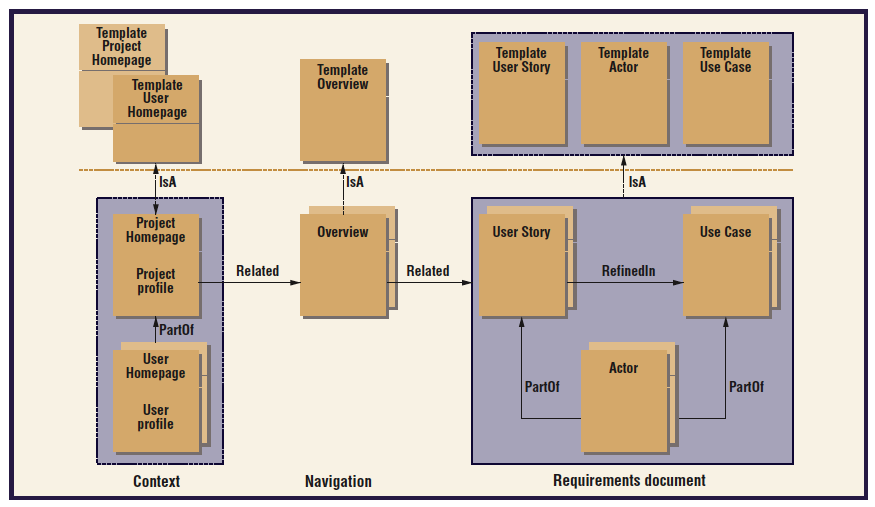
\includegraphics[width=\textwidth]{Wiki.png}
    \caption{A Wiki-Based Document Structure for Requirements Engineering. Source: \cite{wiki_based}}
	\label{fig:wiki}
\end{figure*}

Decker et al. also propose the use of semantic wiki, an approach where additional meta information is used, so that it is possible to reuse the contents using machine learning \cite{self_organized}. In this regard they introduced ``Wikitology'', a term that combines Wiki and Ontology. The Ontology is contained as a part of meta-data in the templates for different software engineering artifacts, such as user stories, discussions, and the like. Once these templates are defined, a software engineering artifact becomes an instance of one of the templates. So, the relationship between two different wiki pages can be established based on their underlying templates' meta information. Given the ontology of different wiki pages, they used two techniques, Latent Semantic Analysis and Case Based Reasoning, to compute the similarity. In this thesis I used the second technique, CBR, to find similarity between an email and a user story. However, instead of using a predefined ontology, Taggy uses the available meta information or context from an email. Also, Taggy combines the context and text similarity in the computation as opposed to solely relying on the context.

Tosic et al. developed Collaborative Semantic Web Portal Prototype. This tool utilizes wiki platform for collaborative knowledge acquisition to be used in agile project management \cite{collaborative_knowledge}. Their solution added access control to the wiki pages and also several indicators for every page such as number of contributors, the creator and so on. Using this system they observed encouraging results such as teamwork and collaboration, open information flow and the light-weight agile vigilance. 

To ease the authoring of wiki pages, OntoWiki incorporates several interesting techniques \cite{ontowiki}. For example, they present a rich editor with support for real-time search from existing content to reduce the time required to produce an article and cross-link with different pages. Also, to make it collaborative they brought the concept of commenting and rating. While these techniques can greatly help in authoring wiki content, to be used in software knowledge management the developers and the customer need to actually put content on the wiki and ensure the content is updated accordingly. This may be a barrier, as it requires dedicating considerable human effort to a cause that has lower immediate business value compared to other tasks, such as developing and testing the software.

Chau et al. studied the contribution to a software wiki made by people working on different roles \cite{a_case_study_of_wiki}. They observed the use of MASE, a wiki-based knowledge sharing system, in a medium-sized software company. They discovered a very high usage of MASE (that exceeds 90\%) as an asynchronous collaboration medium. But surprisingly, only 10\% of the wiki content were produced by the managers, while the rest was contributed by the technical team. Moreover, none of the managers were in the list of top 10 contributors. They also found that there was a greater need for unstructured than structured knowledge. In agile software engineering, informal and continuous customer collaboration is heavily utilized. So, it is important to choose a knowledge sharing media that offers flexibility without a steep learning curve for the customers. This thesis recognizes the need for unstructured knowledge and uses email as a source of such knowledge. As a result, the knowledge base is generated while people communicate as opposed to documented after the knowledge is shared.

Wiki has also been used to write executable acceptance tests with the motivation that customers can provide the acceptance criteria for a user story in simple wiki tables \cite{fitnesse}. For example, Young et al. mentioned the use of wiki for automated acceptance tests so that the continuous integration system could execute the tests\cite{how_did_we}. However, such tabulation of acceptance tests often does not capture underlying knowledge, which may be necessary to understand a user story.

While wikis can work as knowledge sharing tools, the addition of email discussions offer several unique benefits. First, email is a general purpose communication tool, so most people are already familiar with this. Wikis are great for collaborative editing, but knowledge sharing often takes the form of discussion where information flows back and forth between people. For example, it is easier to follow a discussion than to find the latest changes to a  wiki page. As Chau et al. pointed, wikis and similar centralized knowledge capturing approaches often employs people who are not involved in the day-to-day software development and, as a result, there are concerns raised about the usefulness of this approach\cite{a_case_study_of_wiki}. Capturing knowledge from emails and linking it to user stories will complement the collaborative editing benefits of wiki. So, it will add the useful details that are already discussed from emails to any knowledge from the wikis.

\section{Context-Based Knowledge Management}
Maalej et al. provided a context-based solution for lightweight knowledge sharing in distributed software projects \cite{a_lightweight}. They identified two key steps in the knowledge sharing process, namely, knowledge access and knowledge sharing. They outlined a framework to facilitate the access to relevant implicit knowledge from a large amount of dispersed sources. The framework relies on the context of different knowledge items, as well as knowledge consumer's usage pattern, to proactively provide access to the available knowledge. To facilitate knowledge sharing, they identified that a knowledge provider needs to present the knowledge in generalized format so that it can be applied on a different context by another person. This requires additional effort from the provider without much immediate benefit.

To minimize this burden, they proposed the use of additional semantic information or an additional ontology of knowledge items which can be used in computer-based information retrieval through context matching. Their proposed knowledge management solution derives a profile of the developers from their usage history. Based on this profile and the semantic information present at the knowledge artifacts, the relevant ones are found. This proposed solution mainly targets the knowledge capturing at a fragment of source code level. Although this framework provides an abstract form for a knowledge management solution, a concrete description of how the acquisition of dispersed knowledge from sources like emails, wiki, instant messages and forums are incorporated is not discussed. As suggested in this approach, Taggy uses the context information in addition to text relevance to interlink different knowledge items. However, Taggy is designed to capture high level knowledge from emails and user stories as opposed to the level of source code fragments.

\begin{figure*}[ht]
	\centering
	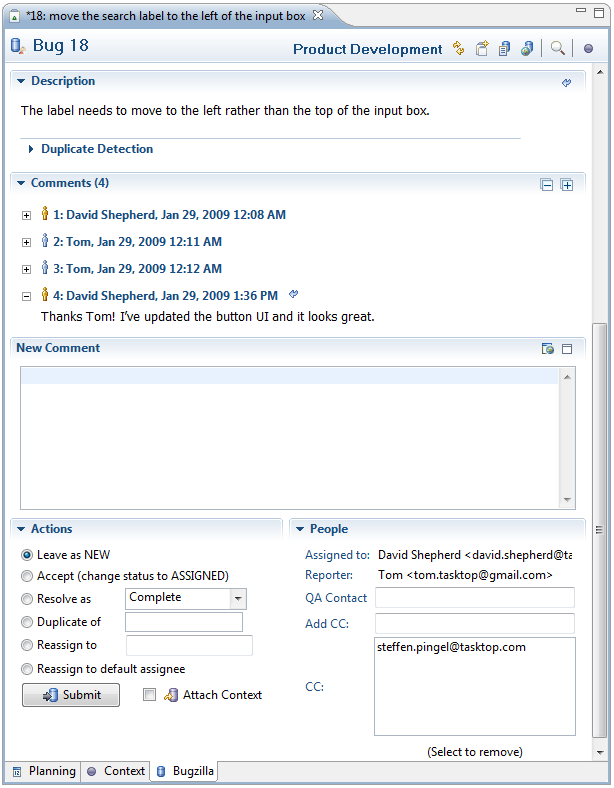
\includegraphics[width=\textwidth]{Mylyn-comment.png}
    \caption{Mylyn Eclipse Plugin - Bugzilla Integration. Source: \cite{mylyn}}
	\label{fig:mylyn}
\end{figure*}

\begin{figure*}[ht]
	\centering
	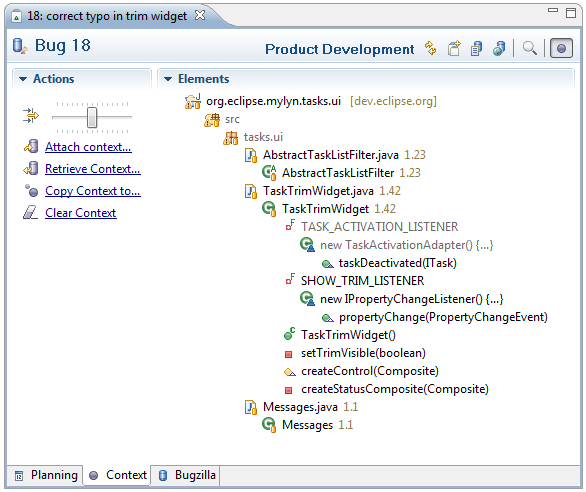
\includegraphics[width=\textwidth]{Mylyn-context.png}
    \caption{Mylyn Eclipse Plugin - Setting source code context of a bug. Source: \cite{mylyn}}
	\label{fig:mylyn}
\end{figure*}

Ratanotayanon et al. developed Zelda, an Integrated Development Environment (IDE) plugin to interlink source code with user stories \cite{supporting_program}. This plugin provides an interface where a developer can select one of the user stories as an active user story. Next, when she is ready to push the changes in the code repository, the plugin automatically links all the changes against the active user story. It also allows a developer to manually select source code that is related to the user story. The goal of this link recording is to help other developers who might need to make changes to the feature from an existing user story. To complete the future modification, one can navigate to relevant source code from the stored links. Since it is a common practice to modify source code and keep revisions, Zelda updates the user story and code links whenever the code has a new revision to keep the links pointed to the latest revision. In their evaluation, they found that Zelda helped developers to focus on relevant source files given a new user story to modify an existing one.

The concept behind Zelda, linking source code changes with requirements and other high level artifacts, is also present in FEAT\cite{feat} and Mylyn\cite{mylyn}. For example, Mylyn is an IDE plugin that builds a task context as developers select a task and make necessary changes. The context of a task includes information about the source code changes, API usage and documentation lookup as a developer works on it. Having this context, a developer can easily navigate and search though relevant source code for a task. Mylyn also has integrations with several task and bug tracking tools. Figure~\ref{fig:mylyn-comment} shows a screenshot of Mylyn where a developer can directly put comments on tasks and browse work items within the IDE while making code changes. Also, they can provide the source context against tasks, so that it is possible to locate the source code for a given task as shown in Figure~\ref{fig:mylyn-context}.

As seen with Zelda and Mylyn, high level artifacts such as user stories and tasks can be used as an entry point to a knowledge base. Taggy follows this same approach. However, instead of linking source code with user stories, Taggy links email discussions. So, the knowledge base produced by Taggy is likely to complement Zelda with relevant higher-level information from emails that can provide greater insight into user stories. In a sense, Taggy interlinks two high level artifacts, which complements the knowledge found from interlinked low level items.

\section{Review of Existing Tool Support for Knowledge Sharing}
Distributed agile projects often use globally available project management tools to share knowledge \cite{essential_communication}. These tools allow the teams to capture the product and iteration backlogs, user stories and project planning information. Typical project planning information includes the estimation and assignment of tasks or user stories to developers and testers. Also, some tools provide support for collaboration about the user stories.

\begin{figure*}[bt]
	\centering
	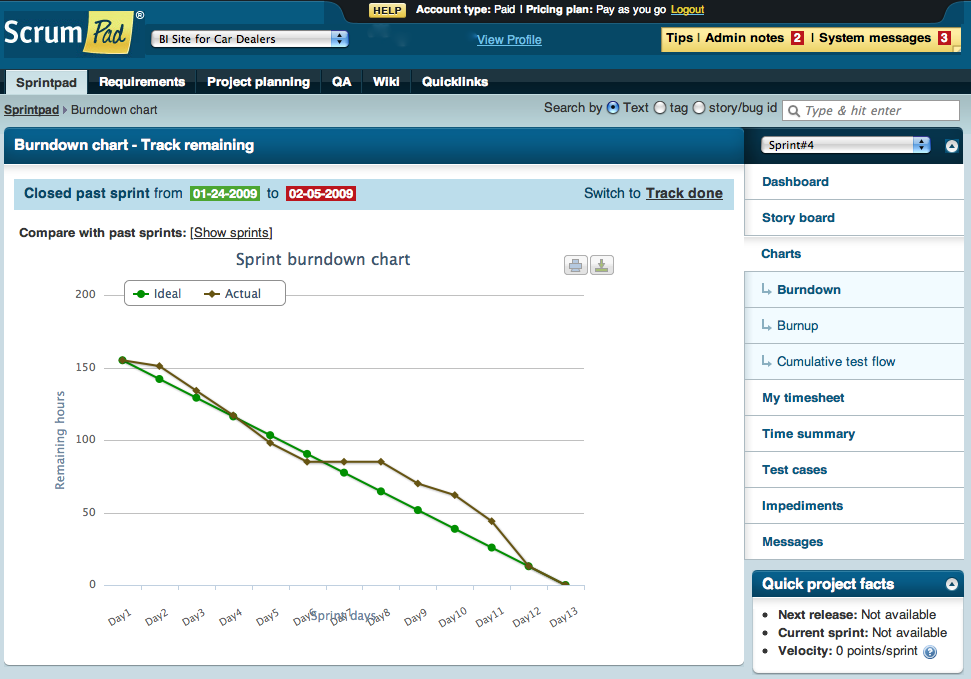
\includegraphics[width=\textwidth]{Scrumpad.png}
    \caption{Dashboard in ScrumPad, a Commercial Agile Project Management Tool. Source: \cite{scrum_pad}}
	\label{fig:scrumpad}
\end{figure*}


There are a number of commercial tools available for agile project management, such as VersionOne\cite{version_one}, Mingle\cite{mingle}, ScrumPad\cite{scrum_pad}, ScrumWorks\cite{scrum_works}, IBM Rational Team Concert\cite{ibm_rtc}. These tools offer templates for capturing various agile software engineering artifacts such as user stories, backlogs, and acceptance tests. Also, they provide process-specific workflows; for example, a workflow for Scrum includes a virtual story wall and various charts for distributed project tracking. Figure~\ref{scrumpad} shows a screen from ScrumPad. As this screen shows, it is possible to search and browse user stories, messages, wikis, etc. as well as produce visual reports on the project's progress using these tools. Some of these tools let people to collaborate using message threads and wiki. These tools are generally useful in planning and tracking activities. In addition to commercial tools, one can also use open-source agile project management tools such as XPlanner\cite{xplanner} and Trac\cite{trac}.

Several issue or bug tracking tools such as Jira\cite{jira}, Bugzilla\cite{bugzilla}, and FogBugz\cite{fog_bugz} are being used in distributed agile projects as well. To support agile processes, these tools offer plugins for agile projects that include some of the features from the aforementioned project management tools. These bug tracking tools provide a messaging system where people can collaborate around bugs. The knowledge shared during this collaboration is often used to solve new bugs\cite{issue_tracking}.

Distributed agile teams often use general purpose project management tools such as Basecamp\cite{basecamp} and Teambox\cite{team_box}. While these tools are not tailored to provide agile-specific artifacts, they are often picked for their simplicity of use. So, instead of providing a template for an user story or an issue, this tools simply provide a to-do list. Similarly, instead of iterations, people rely on milestones. And as seen with other tools, the general purpose web-based project management tools also allow people to use messaging systems to collaborate on their to-do lists.

Alongside project management tools, some distributed agile teams use general purpose shareware tools such as Microsoft SharePoint\cite{share_point}. SharePoint provides an infrastructure for managing websites, communities, content, search and reporting that is mainly configuration-based and does not require coding effort for the most part. In large distributed agile projects, where multiple teams are involved, SharePoint is often used to manage the knowledge.

Some agile projects are now using source code hosting platforms for project management as well. For example, github\cite{github}, CodePlex\cite{codeplex} and similar source code hosting platforms have support for defining issues and user stories. Also, they allow some project planning features, such as iteration backlogs, estimation and assignment of work items.

Agile teams also use continuous integration tools such as Hudson \cite{Hudson}, CruiseControl\cite{cruise_control} and Microsoft Team Server\cite{team_server}. so that the status of the current build is automatically communicated. These tools provide a dashboard and detail view of a project's health that includes build stats, test results and commit history. Distributed agile teams often use a separate tool to capture knowledge about the high level artifacts that are not found in the continuous integration tools.

The aforementioned tools help distributed agile teams to collaborate and share project-related knowledge. Almost all of them send out notification emails when a change takes place, for example, when a user story is assigned or a build succeeds. Such email notification is helpful since it reaches the inbox of people instead of waiting for them to visit the tools. Some of the tools, such as Basecamp and FogBugz, also accept incoming emails from people. But none of the the tools interlinks the incoming emails to the user stories unless a user does it manually. As a result, the benefits of a message thread attached to a user story is not readily available. To ensure the message threads are kept attached to the user stories, the users are forced to use the tools. But, similar to email notification, this could be convenient if a developer or a customer could just send an email to the tool and the tool would automatically attach the email to the relevant user story. Taggy attempts to solve this problem by utilizing the planning information from the project management tools to infer the relevance of an user story against an email.